\section{Integration with Google Maps} 
\label{sec:gmaps} 
 
 
The integration of Google maps onto the system allowed one to create additional features, that aren't available through its commercial service. The Google maps service has limited functionalities for indoor locations. Their functionalities are limited to providing the maps for each floor of the building, providing the possibility of selecting the floor that the user wishes to view and selecting the whole building, which presents the general information relative to it.  
 
 
One of the lacking capacities in our view, is the possibility of selection, i.e. showing markers, within the indoor map. Through the implemented system, this is possible since whenever the location of the user is displayed, it is done through a marker within the indoor map. Another functionality that is provided by the system is the ability to display the user's position on the correct floor. With the Google maps application, even when a building has an indoor map available, the user's position isn't displayed according to its altitude. In a situation where the whole building would be covered by the implemented system, a correct display of the user's movements could be provided. 
 
 
Although the accuracy provided by the implemented system is only room-based, its capable of being improved. Thanks to GEFILOC's architecture, the operation of exchanging/inserting a location algorithm is simple. As such a brief description of how it would be accomplished will be provided. 
 
 
The deployed algorithm can be of different types, depending on the demanded system's location precision. Taking a triangulation algorithm as example, one will now explain the steps required to calculate a position, which can also be seen on figure \ref{fig:algo}. The location algorithm starts by analysing each pair of data individually. For each pair, the ID contained in it is searched for into the beacon manager, so that the received metric can be associated to a physical location. Once the procedure is completed, a complete map of the reference points and their associated distances to the user is obtained. Using the obtained map, an estimation of user's location can be calculated from the three available points. Due to the simplicity of the example, no additional work was conducted. 
 
 
\begin{figure}[H] 
\centering 
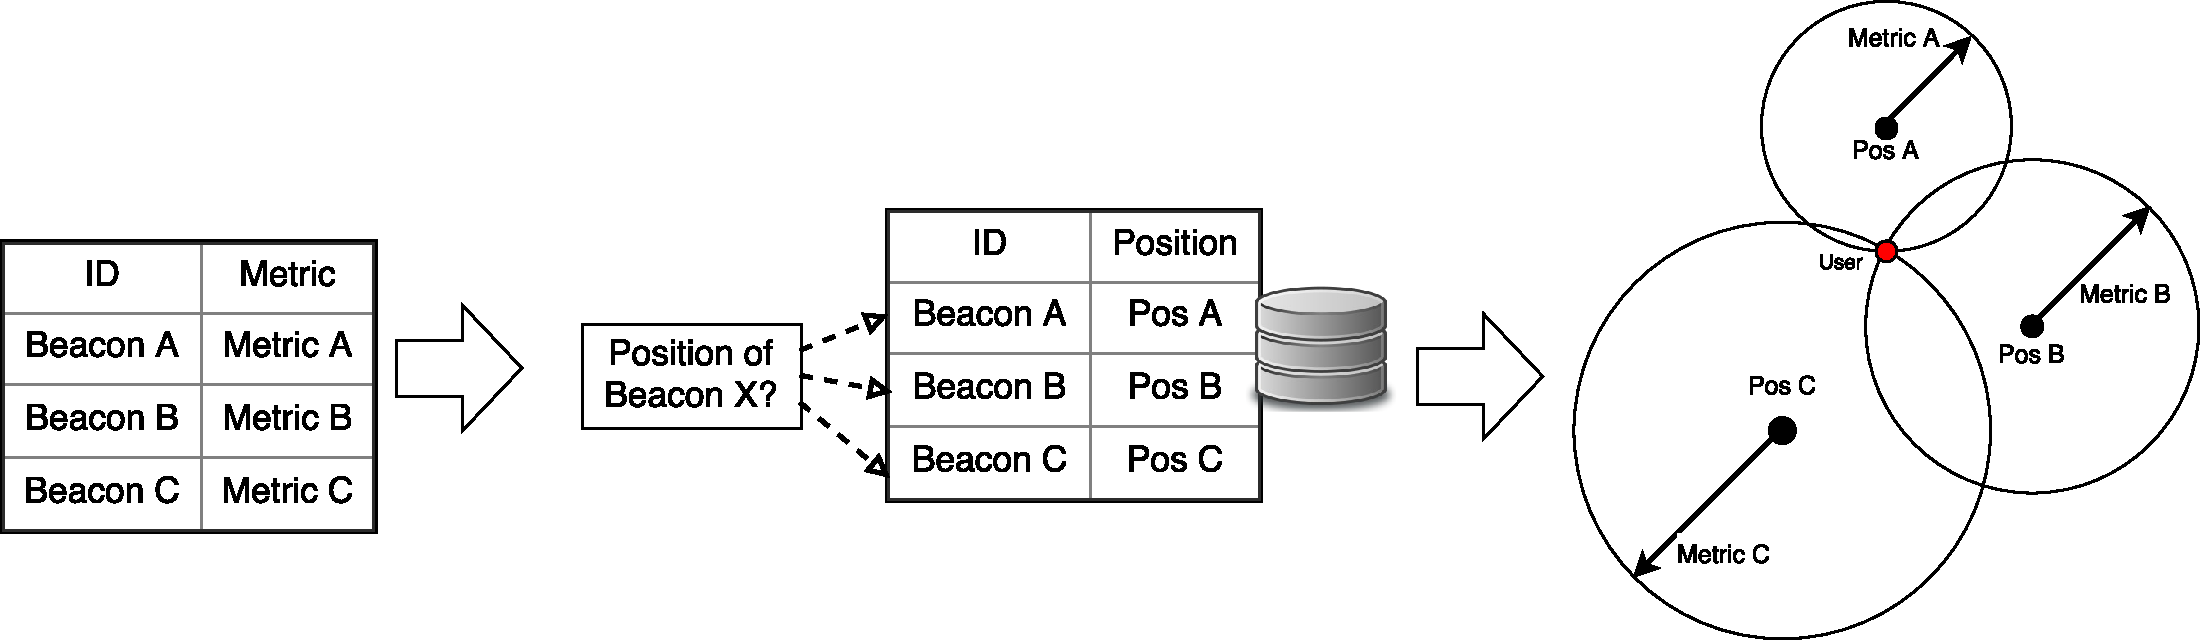
\includegraphics[width=0.9\linewidth]{4.Chapter/Algorithm.pdf} 
\caption[Location algorithm's calculation procedure]{Location algorithm's calculation procedure} 
\label{fig:algo} 
\end{figure} 
 